\documentclass{article}

\usepackage{graphicx}
\usepackage[utf8]{inputenc}

\title{Exabiome Journal}
\author{kellyhuang }
\date{August 2020}

\begin{document}

\maketitle

\section{Roznet Experiments }

\subsubsection*{Small dataset: 200 epochs per run} 

The following experiments were trained with these parameters: 
\newline
-M -g 4 -b 32 -s 3001 -S 1000 -W 1000 --lr 0.001

Roznet on the small dataset, with 5 genomes, achieved a very high accuracy of 96.38\%. There are clear distinctions between each classified genome.  

\begin{figure}[h]
  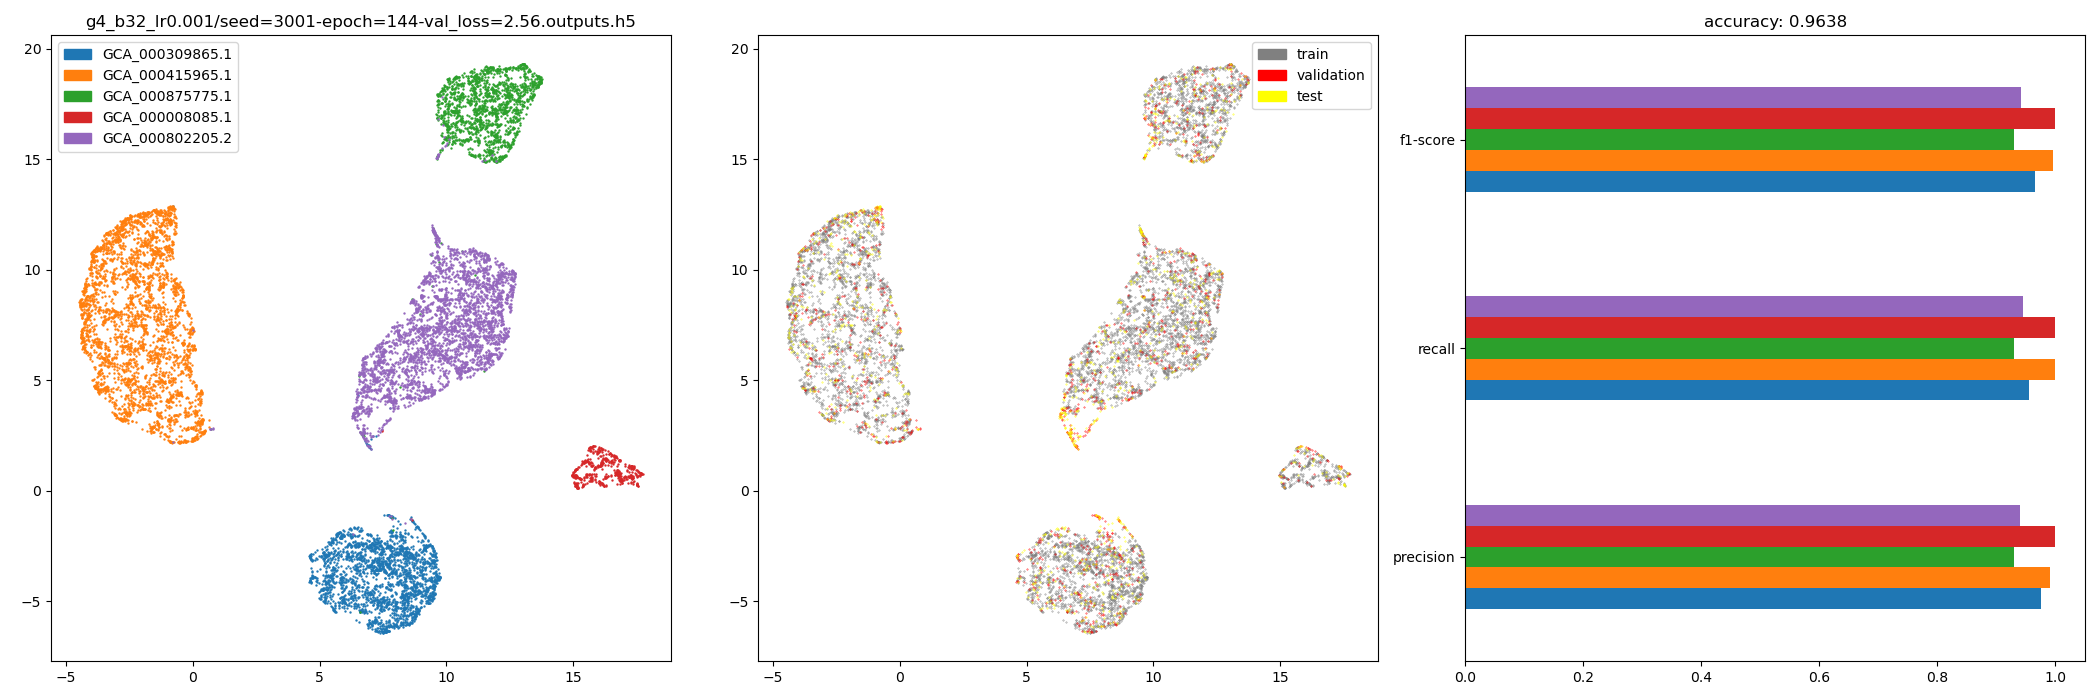
\includegraphics[width=\linewidth]{new_journal/figures/experiments/roznet/small/e200.png}
  \caption{Accuracy: 96.38\%, Best epoch: 144, Validation loss: 2.56}
\end{figure}

\clearpage

\subsubsection*{Medium dataset: 91 epoch per runs}
The following experiments were trained with the following parameters: 
\newline
-M -g 4 -b 32 -s 3001 -S 1000 -W 1000 --lr 0.001

Each 4 hour run reached the maximum time limit at 91 epochs. The best results were achieved on the 124/273 epoch, with an accuracy of 75.37\%. After the second run, the validation loss began to fluctuate back up. Roznet on the medium dataset seems to converge around an accuracy of 75\% after three 91 epoch runs. 

\begin{figure}[h]
  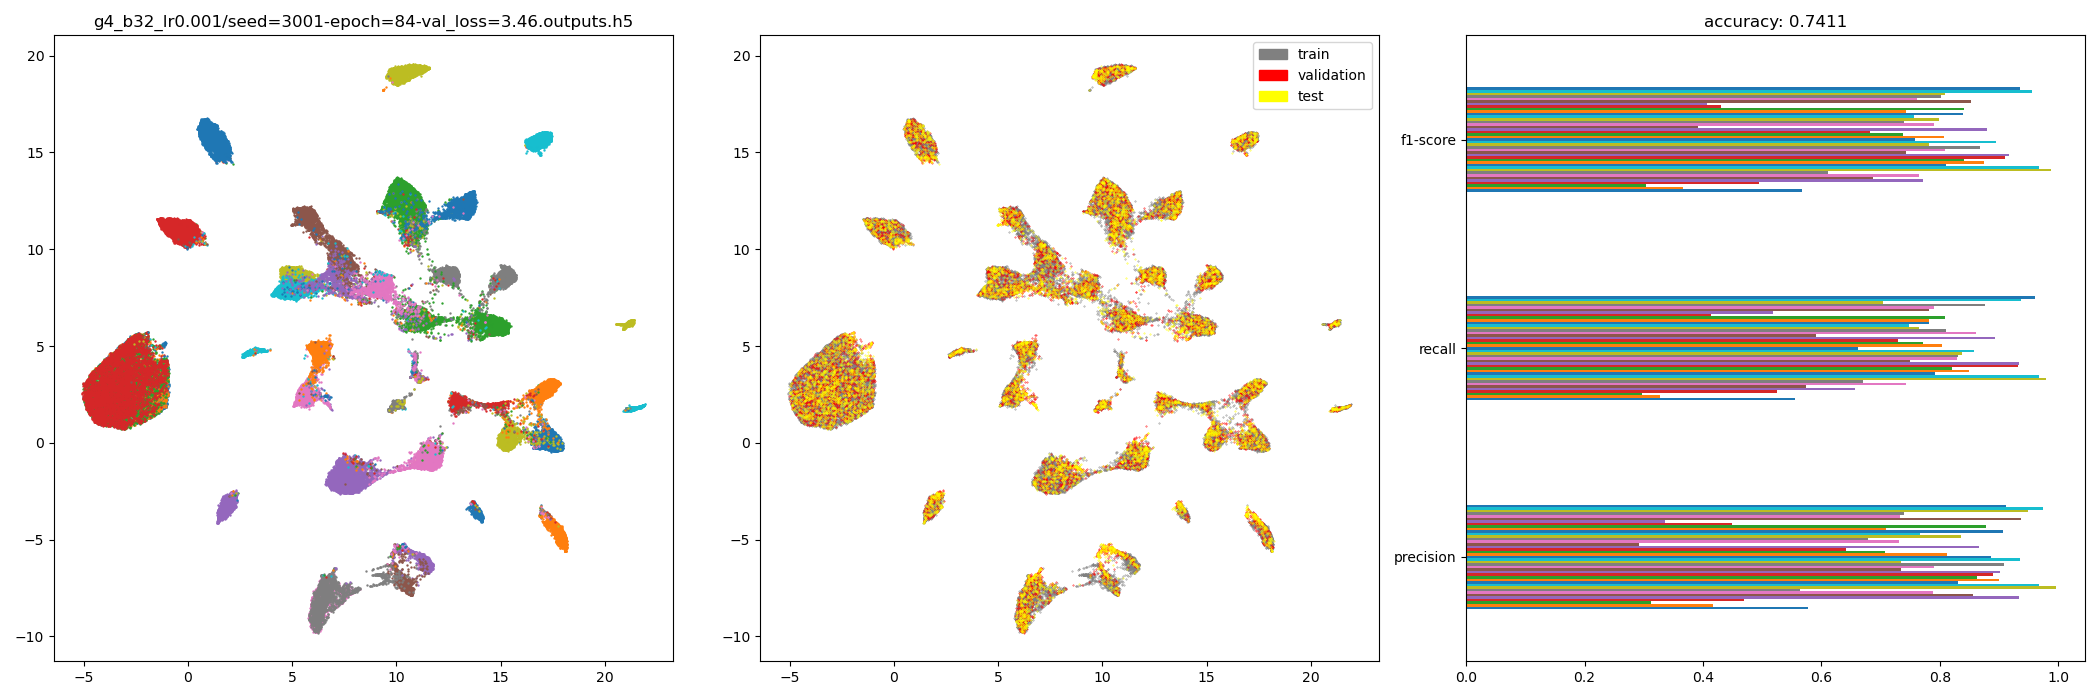
\includegraphics[width=\linewidth]{new_journal/figures/experiments/roznet/medium/lr0.001/run1.png}
  \caption{Run 1 - Accuracy: 74.11\%, Best epoch: 84, Validation loss: 3.46}
\end{figure}

\begin{figure}[h]
  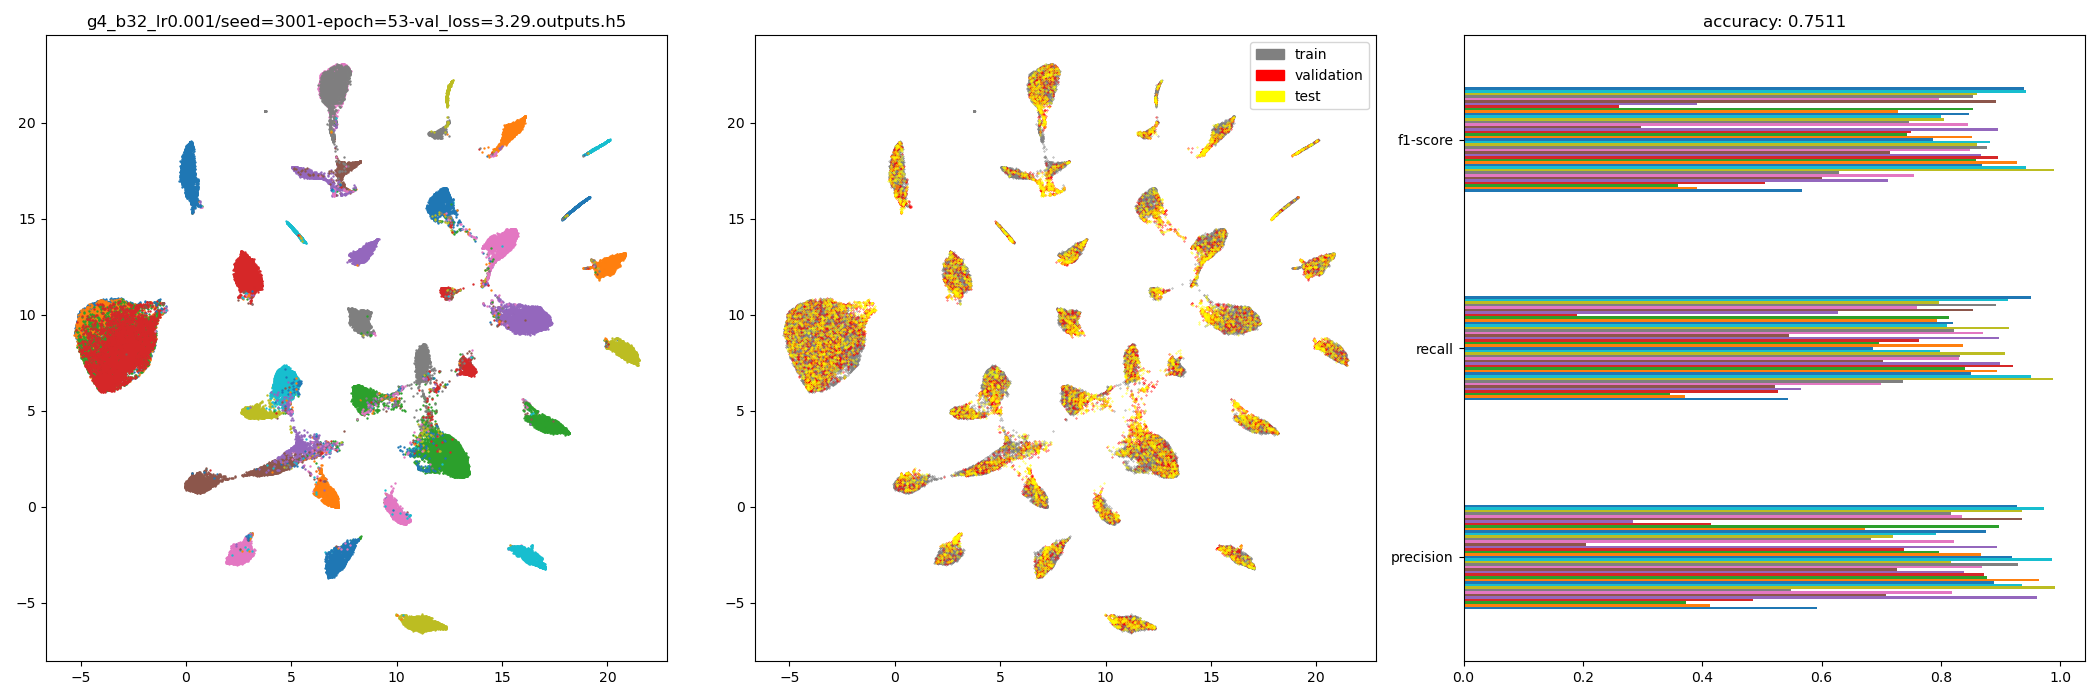
\includegraphics[width=\linewidth]{new_journal/figures/experiments/roznet/medium/lr0.001/run2.png}
  \caption{Run 2 - Accuracy: 0.7537, Best epoch: 33, Validation loss: 3.18}
\end{figure}

\begin{figure}[h]
  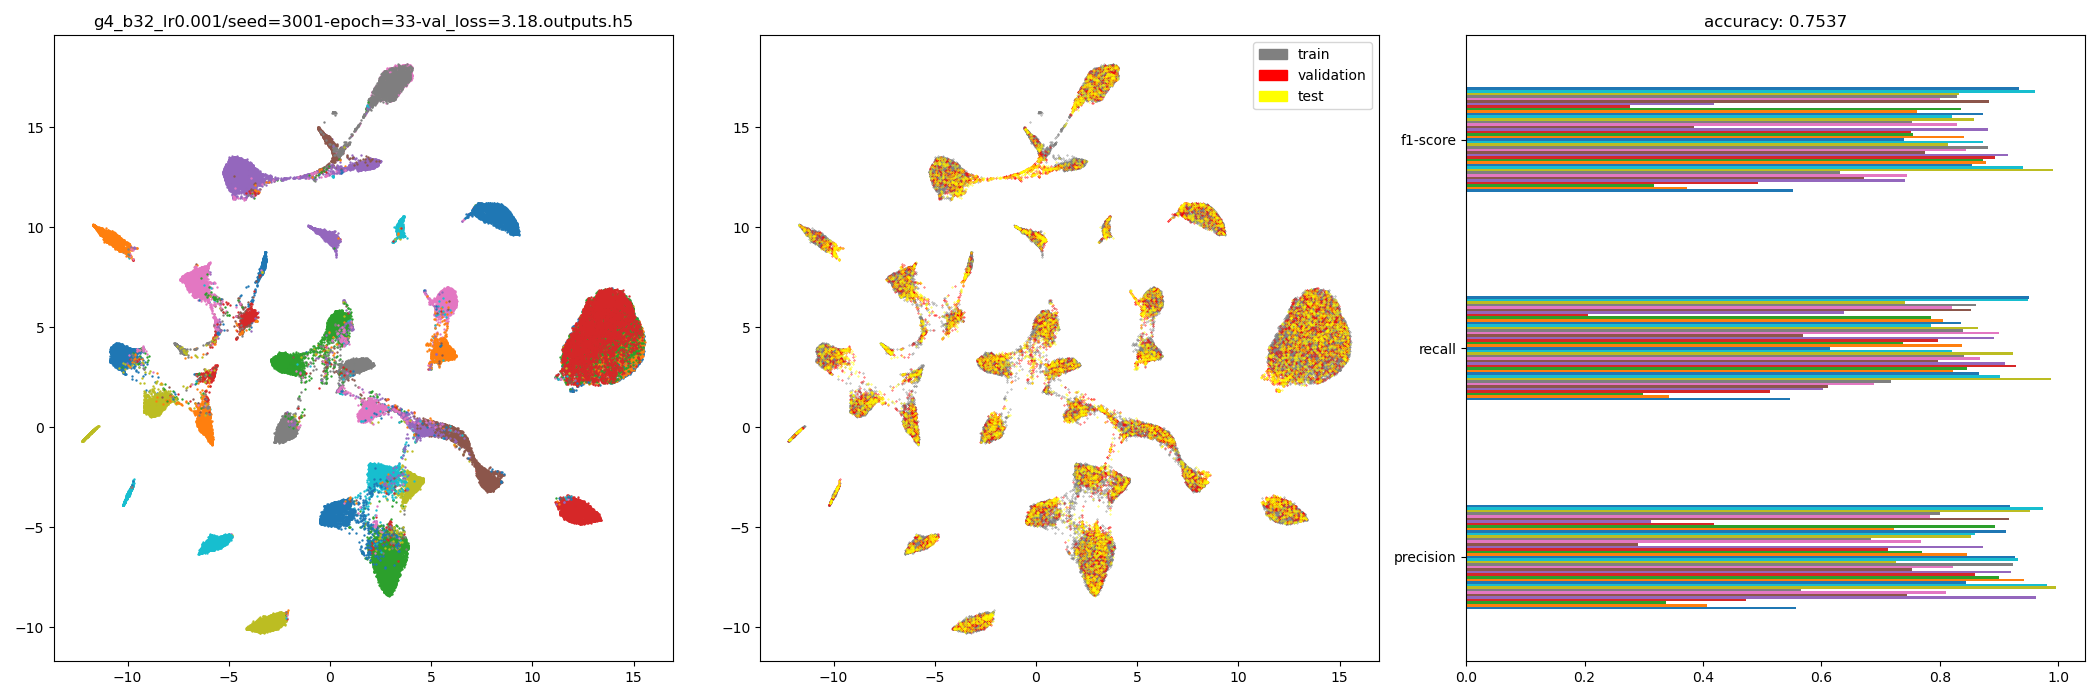
\includegraphics[width=\linewidth]{new_journal/figures/experiments/roznet/medium/lr0.001/run3.png}
  \caption{Run 3 - Accuracy: 75.11\%, Best epoch: 53, Validation loss: 3.29}
\end{figure}

\clearpage

\subsubsection*{Medium dataset: 90 epoch per runs}
The following experiments were trained with the following parameters: 
\newline
-M -g 4 -b 32 -s 3001 -S 1000 -W 1000 --lr 0.0001

\begin{figure}[h]
  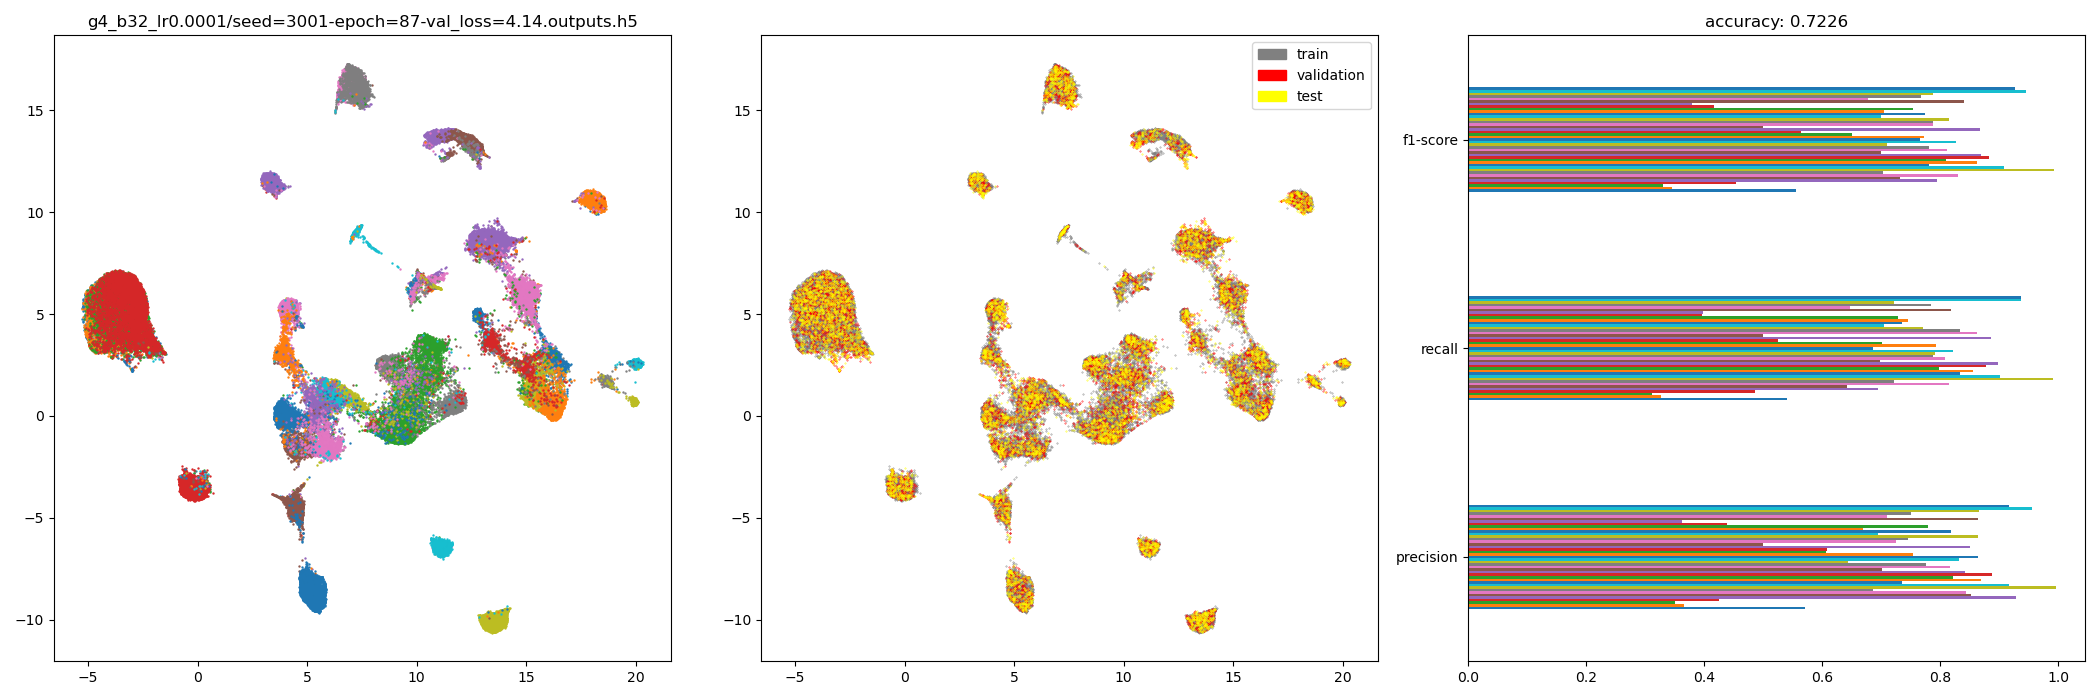
\includegraphics[width=\linewidth]{new_journal/figures/experiments/roznet/medium/lr0.0001/run1.png}
  \caption{Run 1 - Accuracy: 72.36\%, Best epoch: 87, Validation loss: 4.14}
\end{figure}

\subsubsection*{Medium dataset: Varying -S -W}

These experiments were trained with the following parameters: \newline
-M -g 4 -b 32 -s 3001 -S 1000 -W 1000 --lr 0.0001

Using -S 10000 -W 10000 dropped increased the validation loss and decreased the accuracy significantly due to the issue of samples overlapping. Too great of a difference in values between sequence length and window size decreased accuracy. Too large of a sequence length and window size decreased accuracy. The best sequence length and window size was found to be at -S 2000 -W 5000 with an accuracy of 76.47\%.

\begin{figure}[h!]
  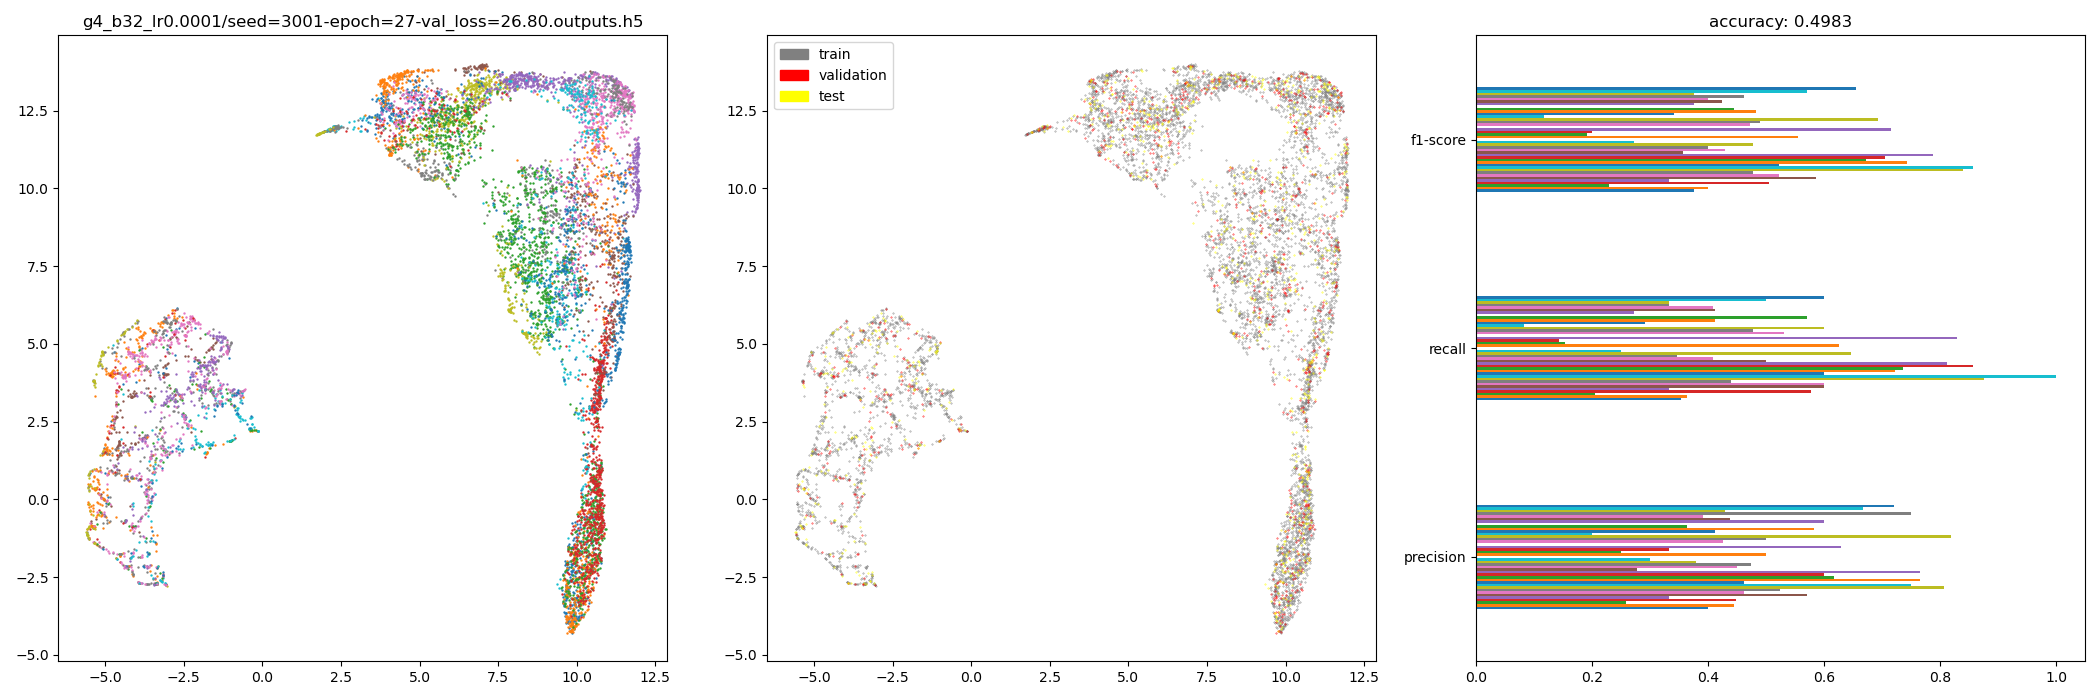
\includegraphics[width=\linewidth]{new_journal/figures/experiments/roznet/medium/S_W/10000_10000.png}
  \caption{-S 10000 -W 10000}
\end{figure}

\begin{figure}[h!]
  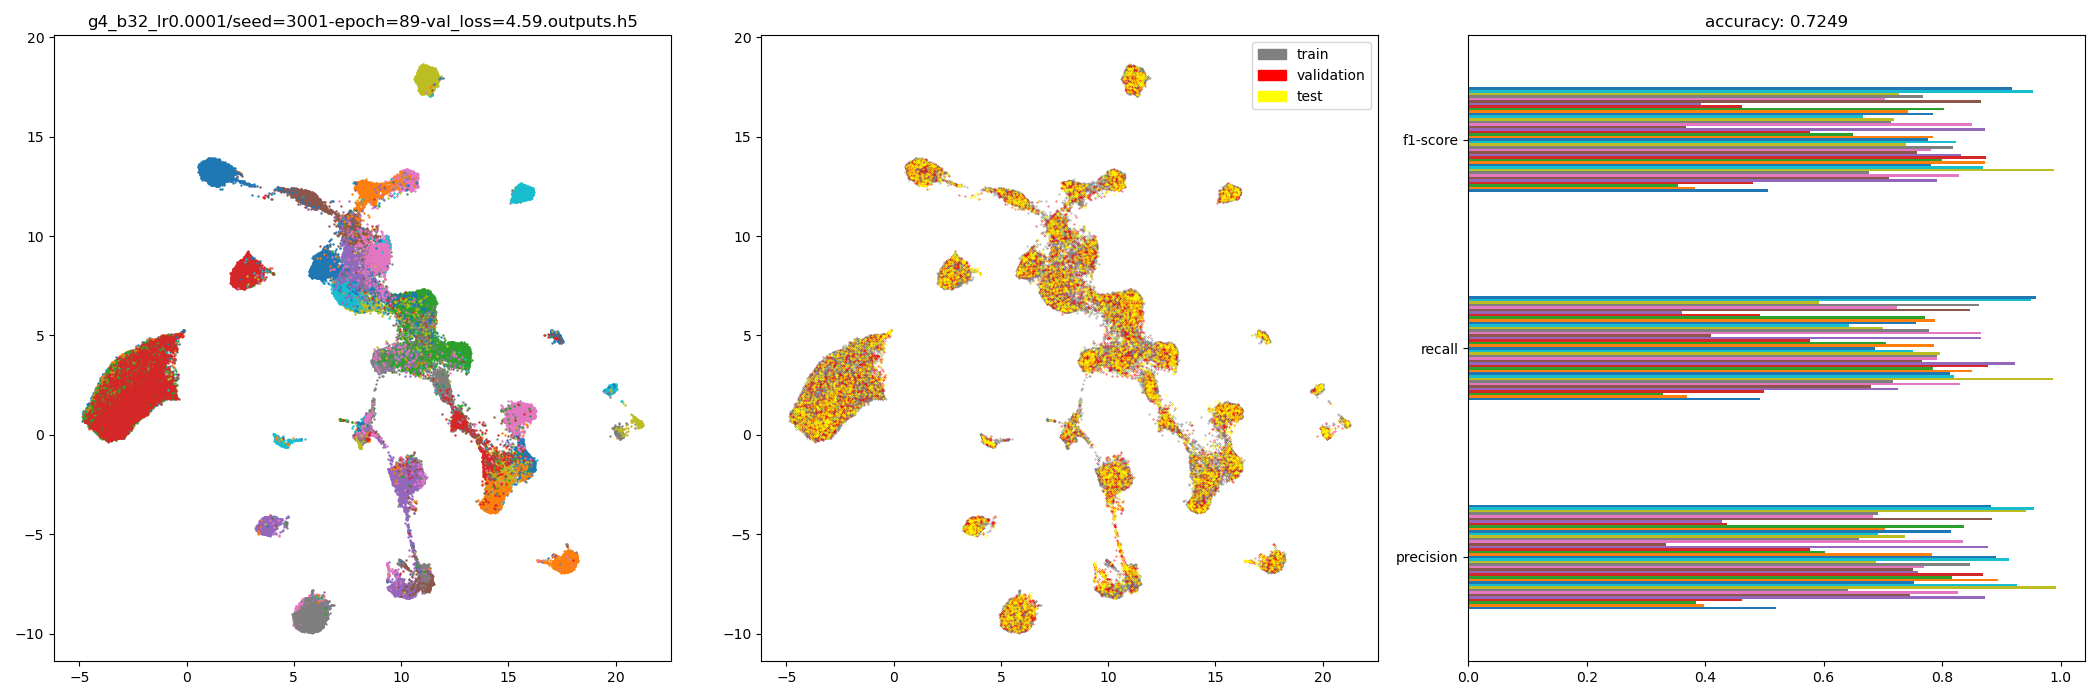
\includegraphics[width=\linewidth]{new_journal/figures/experiments/roznet/medium/S_W/1000_5000.png}
  \caption{-S 1000 -W 5000}
\end{figure}

\begin{figure}[h!]
  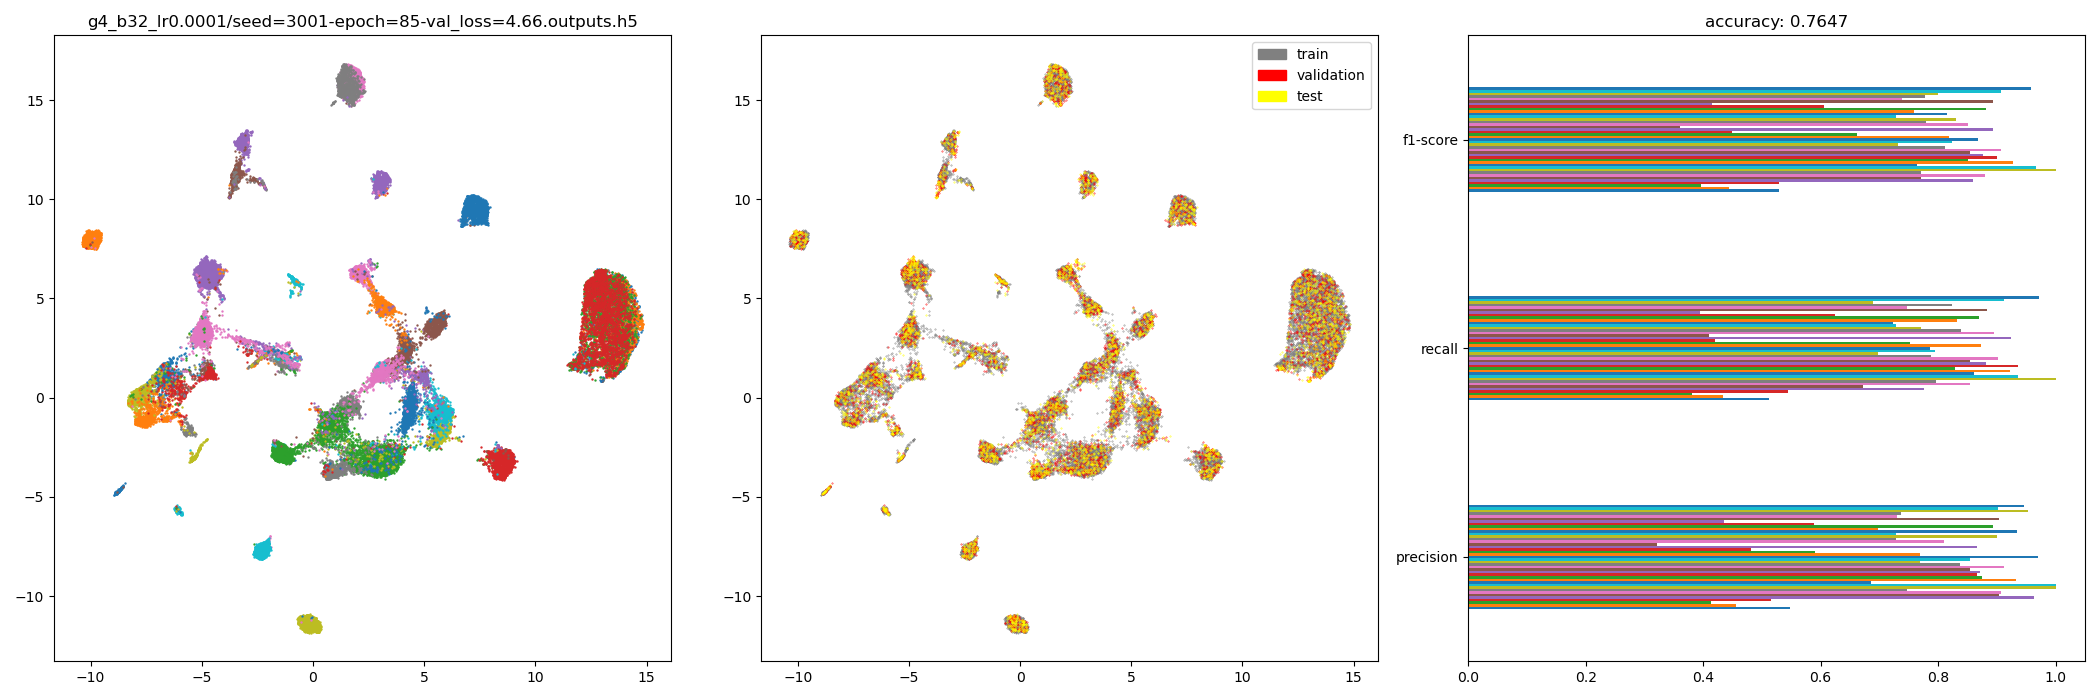
\includegraphics[width=\linewidth]{new_journal/figures/experiments/roznet/medium/S_W/2000_5000.png}
  \caption{-S 2000 -W 5000}
\end{figure}

\begin{figure}[h!]
  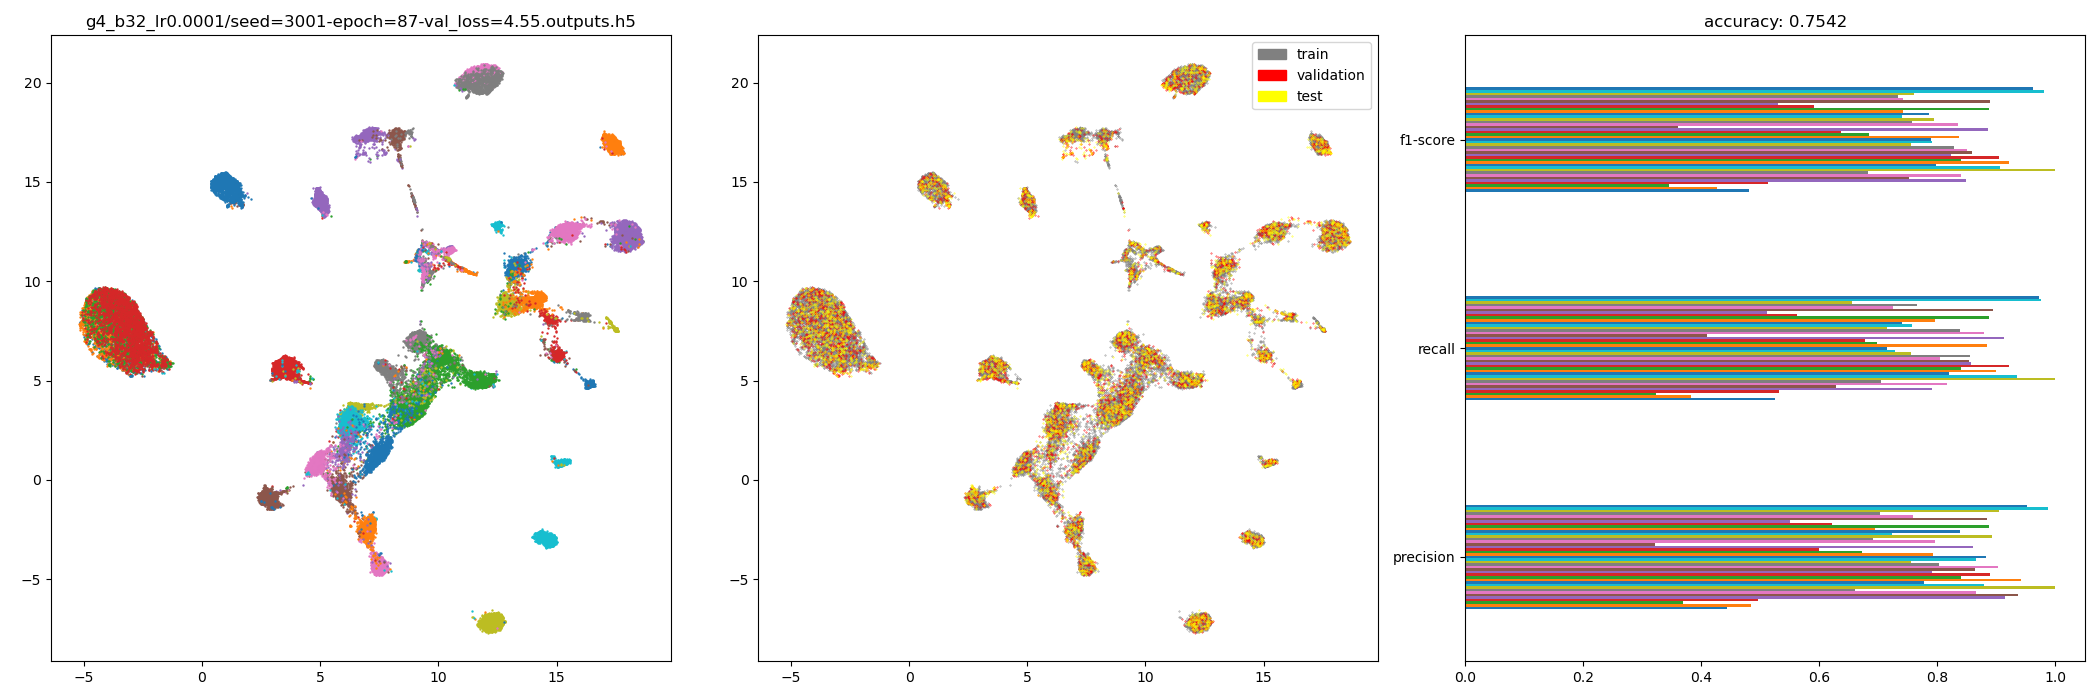
\includegraphics[width=\linewidth]{new_journal/figures/experiments/roznet/medium/S_W/2000_10000.png}
  \caption{-S 2000 -W 10000}
\end{figure}

\begin{figure}[h!]
  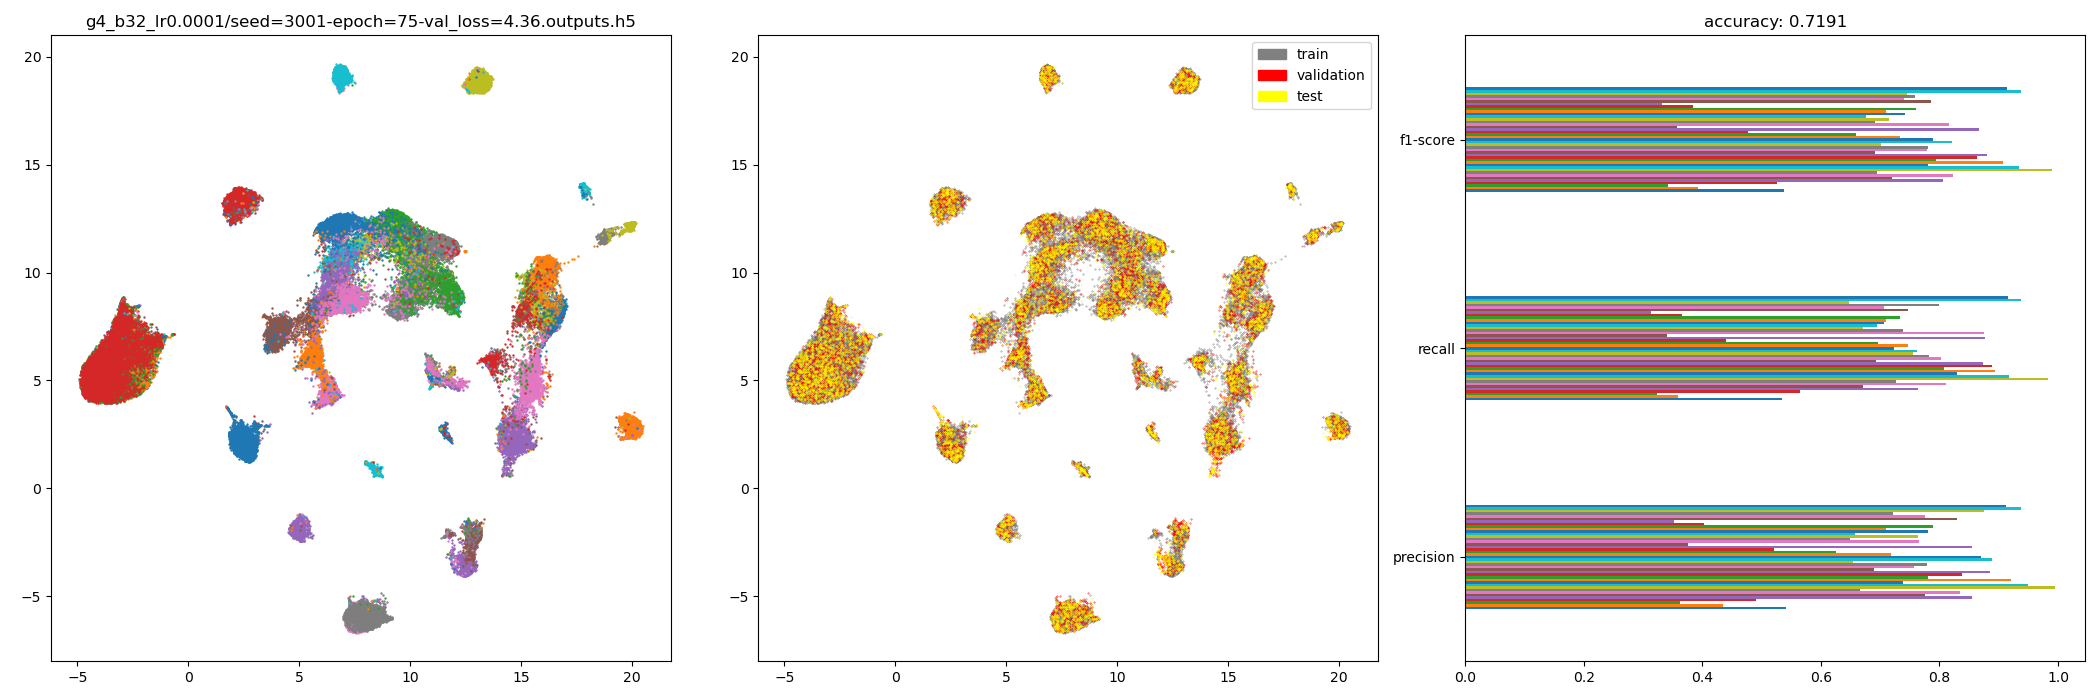
\includegraphics[width=\linewidth]{new_journal/figures/experiments/roznet/medium/S_W/1000_10000.png}
  \caption{-S 1000 -W 10000}
\end{figure}

\begin{figure}[h!]
  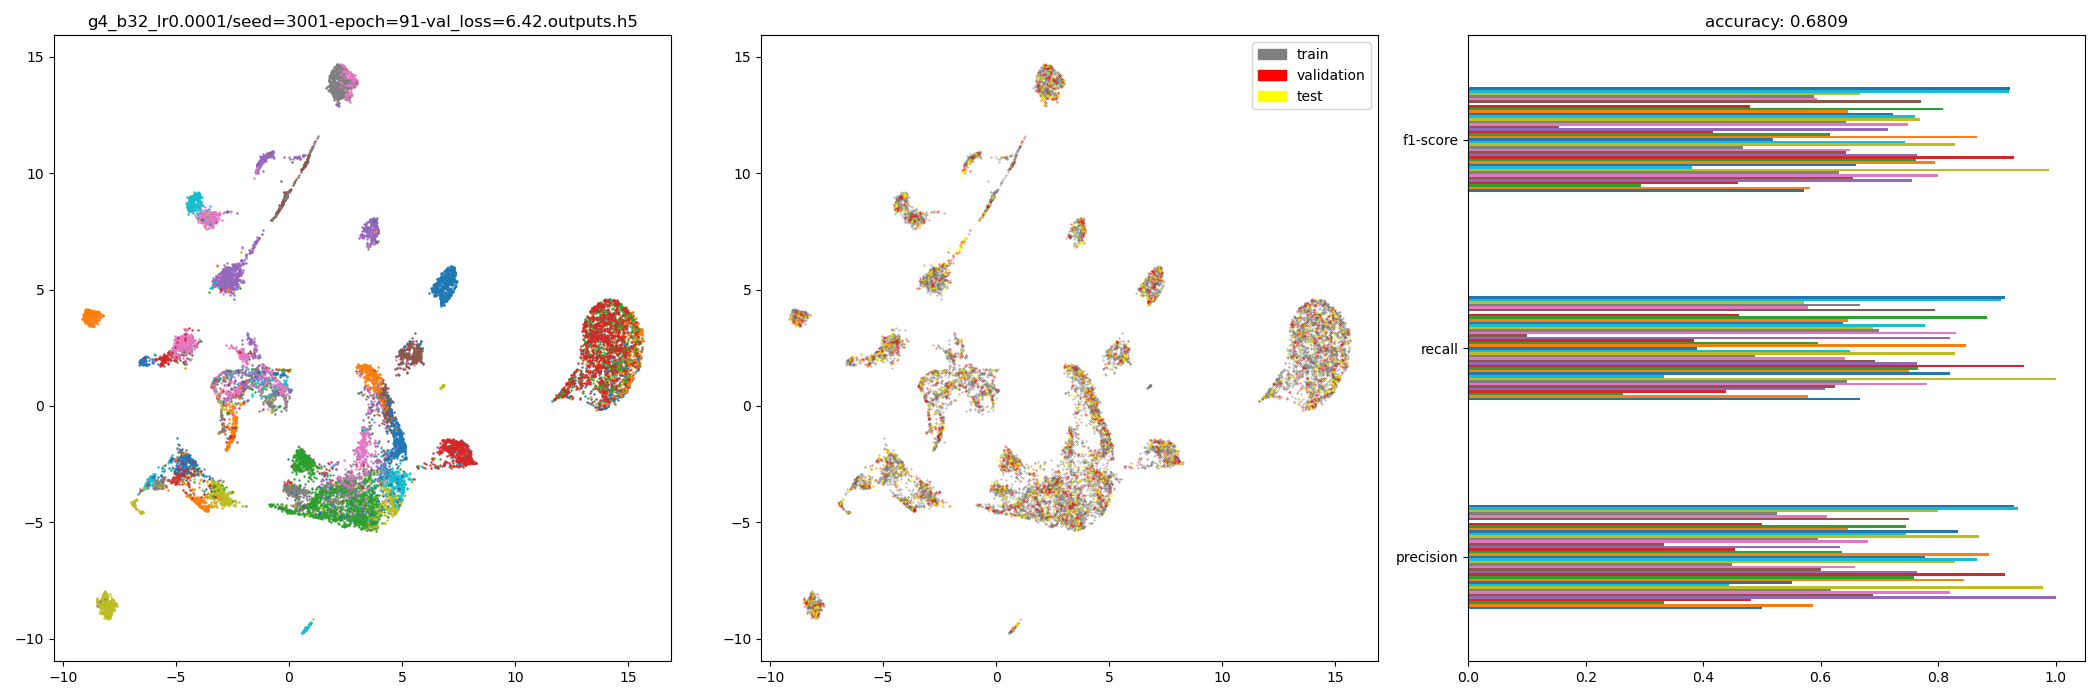
\includegraphics[width=\linewidth]{new_journal/figures/experiments/roznet/medium/S_W/5000_10000.png}
  \caption{-S 5000 -W 10000}
\end{figure}

\end{document}


